\documentclass[11pt,a4paper]{article}

\usepackage[T1]{fontenc}
\usepackage[utf8]{inputenc}
\usepackage{lmodern}
\usepackage[scaled=0.90]{helvet}
\usepackage[a4paper,top=2.1cm,bottom=2.0cm,left=2.4cm,right=2.4cm]{geometry}
\usepackage{microtype}
\linespread{0.96}
\usepackage{parskip}
\setlength{\parskip}{4.8pt plus 1.2pt minus 0.8pt}
\usepackage{graphicx}
\usepackage{xcolor}
\usepackage{booktabs}
\usepackage{array}
\usepackage{longtable}
\usepackage{caption}
\usepackage{float}
\usepackage{listings}
\usepackage{titlesec}
\usepackage{fancyhdr}
\usepackage{tikz}
\usetikzlibrary{arrows.meta,shapes.multipart,positioning,calc,fit,backgrounds}
\usepackage[colorlinks=true,linkcolor=linkblue,urlcolor=linkblue,citecolor=linkblue]{hyperref}

% ---------------------------------------------------------------- palette --
\definecolor{linkblue}{HTML}{1F4E79}
\definecolor{rule}{HTML}{C8CED6}

\definecolor{cActorF}{HTML}{E9EDF1}\definecolor{cActorL}{HTML}{5B6B7C}
\definecolor{cCliF}{HTML}{FBEEDB}  \definecolor{cCliL}{HTML}{9D6D28}
\definecolor{cBffF}{HTML}{DDE8F7}  \definecolor{cBffL}{HTML}{3A6596}
\definecolor{cApiF}{HTML}{D8ECDC}  \definecolor{cApiL}{HTML}{3F7A4F}
\definecolor{cDbF}{HTML}{E7E1F4}   \definecolor{cDbL}{HTML}{5D489A}
\definecolor{cBar}{HTML}{DCE3E9}
\definecolor{cNote}{HTML}{F4F6F8}
\definecolor{cLost}{HTML}{B03A34}
\definecolor{cCode}{HTML}{F6F7F9}

% ---------------------------------------------------------------- headings --
\titleformat{\section}{\sffamily\large\bfseries}{\thesection}{0.7em}{}
\titleformat{\subsection}{\sffamily\normalsize\bfseries}{\thesubsection}{0.7em}{}
\titlespacing*{\section}{0pt}{14pt plus 3pt minus 3pt}{5pt}
\titleformat{\subsubsection}{\sffamily\normalsize\bfseries}{\thesubsubsection}{0.7em}{}
\titlespacing*{\subsection}{0pt}{10pt plus 2pt minus 2pt}{3pt}
\titlespacing*{\subsubsection}{0pt}{11pt plus 2pt minus 1pt}{3pt}
\newcolumntype{R}[1]{>{\raggedright\arraybackslash}p{#1}}

\pagestyle{fancy}\fancyhf{}
\renewcommand{\headrulewidth}{0pt}
\fancyfoot[C]{\sffamily\footnotesize\color{black!55}\thepage}

\captionsetup{font={sf,small},labelfont={sf,small,bf},skip=5pt,width=0.94\textwidth}
\setlength{\emergencystretch}{3em}
\setlength{\LTcapwidth}{\textwidth}
\setlength{\tabcolsep}{5pt}
\renewcommand{\arraystretch}{1.18}

% ---------------------------------------------------------------- listings --
\lstdefinestyle{code}{
  basicstyle=\ttfamily\fontsize{7.6}{9.1}\selectfont,
  keywordstyle=\color{cBffL}\bfseries,
  commentstyle=\color{black!45}\itshape,
  stringstyle=\color{cApiL!80!black},
  backgroundcolor=\color{cCode},
  frame=leftline, framerule=1.2pt, rulecolor=\color{rule},
  framesep=6pt, xleftmargin=8pt, aboveskip=6pt, belowskip=4pt,
  breaklines=true, breakatwhitespace=true, columns=fullflexible,
  keepspaces=true, showstringspaces=false, tabsize=2,
  morekeywords={await,async,var,public,private,static,return,new,using,null,
    catch,try,class,if,else,throw,const,export,function,type,import,from,
    SELECT,FROM,WHERE,UPDATE,INSERT,COMMIT,ROLLBACK,BEGIN,FOR,KEY,SHARE,NO}
}
\lstset{style=code}

% -------------------------------------------------- sequence diagram tools --
\def\sqbot{-8}
\tikzset{
  sqhead/.style={draw,rounded corners=1.5pt,align=center,
      font=\sffamily\fontsize{7}{8}\selectfont,minimum height=8mm,
      minimum width=15mm,inner xsep=3pt,line width=0.5pt},
  sqactor/.style={sqhead,fill=cActorF,draw=cActorL},
  sqclient/.style={sqhead,fill=cCliF,draw=cCliL},
  sqbff/.style={sqhead,fill=cBffF,draw=cBffL},
  sqapi/.style={sqhead,fill=cApiF,draw=cApiL},
  sqdb/.style={sqhead,fill=cDbF,draw=cDbL},
  sqline/.style={dash pattern=on 2pt off 2.4pt,draw=black!32,line width=0.4pt},
  sqmsg/.style={-{Stealth[length=3.8pt,width=2.8pt]},line width=0.55pt,draw=black!80},
  sqret/.style={-{Stealth[length=3.8pt,width=2.8pt]},line width=0.5pt,draw=black!52,
      dash pattern=on 2.4pt off 1.8pt},
  sqlab/.style={font=\sffamily\fontsize{6.4}{7.2}\selectfont,midway,above=0.4pt,
      inner sep=1pt,fill=white,text=black!84,align=center},
  sqfree/.style={font=\sffamily\fontsize{6.4}{7.2}\selectfont,inner sep=1pt,
      fill=white,text=black!84,align=left},
  sqfrag/.style={draw=cBffL!55,line width=0.4pt},
  notebox/.style={draw=cActorL!45,fill=cNote,line width=0.4pt,rounded corners=1pt,
      font=\sffamily\fontsize{6.4}{7.6}\selectfont,text=black!70,inner sep=4pt,align=left},
  boxy/.style={draw,rounded corners=2pt,align=center,line width=0.6pt,
      font=\sffamily\fontsize{7.4}{8.8}\selectfont,inner sep=5pt},
}

% #1 x  #2 node  #3 style  #4 title  #5 subtitle
\newcommand{\lifeline}[5]{%
  \node[#3,anchor=north] (#2) at (#1,0)
    {\textbf{#4}\\[-1.5pt]{\fontsize{5.8}{6.4}\selectfont #5}};
  \draw[sqline] (#1,-0.82) -- (#1,\sqbot);}
% #1 x1  #2 x2  #3 y  #4 label
\newcommand{\msg}[4]{\draw[sqmsg] (#1,#3) -- (#2,#3) node[sqlab]{#4};}
\newcommand{\ret}[4]{\draw[sqret] (#1,#3) -- (#2,#3) node[sqlab]{#4};}
% #1 x  #2 y  #3 label
\newcommand{\selfmsg}[3]{%
  \draw[sqmsg] (#1,#2) -- (#1+0.38,#2) -- (#1+0.38,#2-0.3) -- (#1,#2-0.3);
  \node[sqfree,anchor=west] at (#1+0.48,#2-0.15) {#3};}
% #1 x  #2 ytop  #3 ybottom
\newcommand{\act}[3]{\fill[cBar,draw=black!28,line width=0.3pt]
  (#1-0.055,#2) rectangle (#1+0.055,#3);}
% #1 x1  #2 ytop  #3 x2  #4 ybottom  #5 kind  #6 guard
\newcommand{\frag}[6]{%
  \draw[sqfrag] (#1,#2) rectangle (#3,#4);
  \filldraw[sqfrag,fill=white] (#1,#2) -- (#1+0.72,#2) -- (#1+0.72,#2-0.26)
    -- (#1,#2-0.26) -- cycle;
  \node[font=\sffamily\fontsize{5.8}{6.4}\selectfont\bfseries,text=black!58]
    at (#1+0.36,#2-0.13) {#5};
  \node[font=\sffamily\fontsize{6}{6.8}\selectfont\itshape,text=black!58,anchor=west]
    at (#1+0.82,#2-0.13) {#6};}
% #1 x1  #2 x2  #3 fill  #4 label
\newcommand{\band}[4]{%
  \filldraw[fill=#3,draw=#3!72!black,line width=0.35pt,rounded corners=1.5pt]
    (#1,0.66) rectangle (#2,0.26);
  \node[font=\sffamily\fontsize{6.2}{7}\selectfont\bfseries,text=black!62]
    at ({0.5*(#1+#2)},0.46) {#4};}
% #1 x  #2 y  #3 width  #4 text
\newcommand{\sqnote}[4]{\node[notebox,text width=#3,anchor=north west] at (#1,#2) {#4};}
% #1 x  #2 y
\newcommand{\dest}[2]{\draw[line width=0.8pt,draw=cLost]
  (#1-0.13,#2+0.13)--(#1+0.13,#2-0.13) (#1-0.13,#2-0.13)--(#1+0.13,#2+0.13);}
% #1 x1  #2 x2  #3 y  #4 label   (lost message: stops at a filled dot)
\newcommand{\lost}[4]{\draw[sqmsg,draw=cLost,-{Circle[length=3.4pt]}]
  (#1,#3) -- (#2,#3) node[sqlab,text=cLost]{#4};}

\newcommand{\code}[1]{\texttt{\fontsize{8.6}{10}\selectfont #1}}
\newcommand{\actorfig}[2]{%
  \draw[draw=cActorL,line width=0.55pt] (#1,-0.17) circle (0.135);
  \draw[draw=cActorL,line width=0.55pt] (#1,-0.31)--(#1,-0.58)
    (#1-0.18,-0.40)--(#1+0.18,-0.40) (#1,-0.58)--(#1-0.15,-0.80)
    (#1,-0.58)--(#1+0.15,-0.80);
  \node[font=\sffamily\fontsize{6.6}{7.4}\selectfont,text=black!78,anchor=north]
    at (#1,-0.84) {#2};
  \draw[sqline] (#1,-1.06) -- (#1,\sqbot);}
\newcommand{\brk}{\discretionary{}{}{}}
\newcommand{\sub}[1]{{\fontsize{6.2}{7.2}\selectfont #1}}

\begin{document}
% ================================================================= TITLE ==
\thispagestyle{fancy}
\begin{center}
  {\sffamily\fontsize{20}{24}\selectfont\bfseries Mini Transaction Ledger}\\[3pt]
  {\sffamily\fontsize{11}{13}\selectfont\color{black!60}
   Architecture, code structure, API internals and Docker setup}\\[10pt]
  {\sffamily\fontsize{11}{13}\selectfont Abir Rahman}\\[4pt]
  {\sffamily\fontsize{8.6}{11}\selectfont
   \href{mailto:abirr7140@gmail.com}{abirr7140@gmail.com}
   \;\textcolor{rule}{\textbar}\;
   \href{https://www.linkedin.com/in/abir-rahman-059169264/}{linkedin.com/in/abir-rahman-059169264}
   \;\textcolor{rule}{\textbar}\;
   \href{https://github.com/abirzishan32}{github.com/abirzishan32}}
\end{center}
\vspace{2pt}
{\color{rule}\hrule height 0.6pt}
\vspace{10pt}

% ================================================================ SECTION 1
\section{System overview}

The application maintains a double entry ledger for a single authenticated
user. Each user holds a private chart of accounts, posts transactions against
those accounts, and retrieves balances, per account statements and a trial
balance. No data is shared between users and the system defines no
administrative role.

Double entry requires that every transaction affect exactly two accounts. Value
leaves one account and arrives at the other, so a posting is recorded as two
rows whose amounts sum to zero. The schema declares no separate debit and credit
columns. A single signed \code{Amount} carries both senses: a positive value is
a debit and a negative value is a credit. A consulting fee of 250.00 received
into Cash is stored as \code{+250.00} against Cash and \code{-250.00} against
Consulting Income.

Balances are not stored. The balance of an account is defined as
\code{SUM(Amount)} over the entries that reference it, evaluated when the value
is requested. A stored balance would constitute a second representation of a
fact the entries already hold, and two representations of one fact diverge over
time. Deriving the balance removes that class of defect entirely.


% ================================================================ SECTION 2
\section{Application architecture}

The system has four parts: the browser, the frontend, which is a Next.js server
that renders pages and holds the session, the backend, which is an ASP.NET Core
API that owns every rule, and the database. Figure~\ref{fig:arch} states the
components of each and the traffic that passes between them.

\subsection{Separation of the frontend and the backend}

The browser does not communicate with the ASP.NET Core API. It communicates
with a Next.js server, which issues the corresponding request to the API on the
user's behalf. This arrangement is known as a backend for frontend.

The determining factor is the access token. A browser calling the API directly
would have to hold a JSON Web Token, and every storage location a browser
offers is readable by any script on the page: \code{localStorage},
\code{sessionStorage} and cookies without the \code{HttpOnly} attribute are all
exposed to a cross site scripting defect. The Next.js server therefore holds
both tokens as \code{HttpOnly} cookies, which the browser transmits
automatically but never exposes to JavaScript. The token is read from the cookie
in \code{lib/auth.ts} and attached to the outbound request in \code{lib/api.ts},
and is never serialised into markup.

Two further properties follow from this separation. The address of the API is
held in a server side environment variable, \code{API\_BASE\_URL}, which carries
no \code{NEXT\_PUBLIC\_} prefix and is consequently not addressable from a
browser. In addition, \code{lib/api.ts} and \code{lib/auth.ts} both import
\code{server-only} on their first line, which converts any attempt to import
them from a client component into a compilation failure rather than a runtime
disclosure.

\begin{figure}[H]
\centering
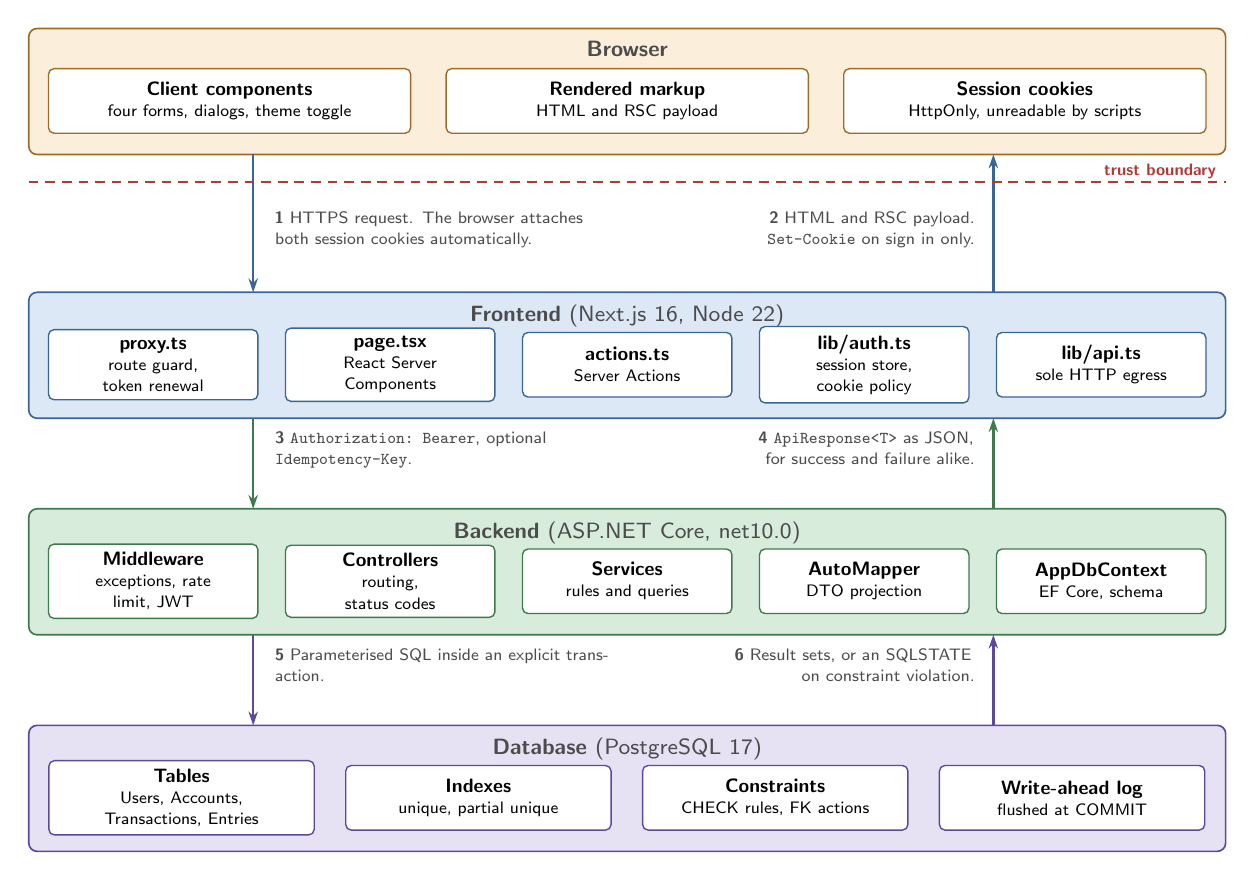
\begin{tikzpicture}[x=1cm,y=1cm,
  tier/.style={rounded corners=3pt,line width=0.6pt},
  thead/.style={font=\sffamily\fontsize{7.6}{9}\selectfont\bfseries,text=black!70,anchor=north},
  comp/.style={draw,rounded corners=2pt,line width=0.5pt,fill=white,align=center,
    font=\sffamily\fontsize{6.6}{7.6}\selectfont,minimum height=0.82cm,inner sep=3pt},
  flow/.style={-{Stealth[length=5pt,width=3.4pt]},line width=0.9pt},
  fl/.style={font=\sffamily\fontsize{6.4}{7.6}\selectfont,text=black!70,inner sep=2pt}]

  \filldraw[tier,fill=cCliF,draw=cCliL] (0.15,0) rectangle (15.35,-1.60);
  \filldraw[tier,fill=cBffF,draw=cBffL] (0.15,-3.35) rectangle (15.35,-4.95);
  \filldraw[tier,fill=cApiF,draw=cApiL] (0.15,-6.10) rectangle (15.35,-7.70);
  \filldraw[tier,fill=cDbF,draw=cDbL]   (0.15,-8.85) rectangle (15.35,-10.45);

  \node[thead] at (7.75,-0.04) {Browser};
  \node[thead] at (7.75,-3.39) {Frontend {\mdseries(Next.js 16, Node 22)}};
  \node[thead] at (7.75,-6.14) {Backend {\mdseries(ASP.NET Core, net10.0)}};
  \node[thead] at (7.75,-8.89) {Database {\mdseries(PostgreSQL 17)}};

  \node[comp,draw=cCliL,minimum width=4.60cm] at (2.70,-0.92)
    {\textbf{Client components}\\\sub{four forms, dialogs, theme toggle}};
  \node[comp,draw=cCliL,minimum width=4.60cm] at (7.75,-0.92)
    {\textbf{Rendered markup}\\\sub{HTML and RSC payload}};
  \node[comp,draw=cCliL,minimum width=4.60cm] at (12.80,-0.92)
    {\textbf{Session cookies}\\\sub{HttpOnly, unreadable by scripts}};

  \node[comp,draw=cBffL,minimum width=2.66cm] at (1.73,-4.27)
    {\textbf{proxy.ts}\\\sub{route guard,}\\\sub{token renewal}};
  \node[comp,draw=cBffL,minimum width=2.66cm] at (4.74,-4.27)
    {\textbf{page.tsx}\\\sub{React Server}\\\sub{Components}};
  \node[comp,draw=cBffL,minimum width=2.66cm] at (7.75,-4.27)
    {\textbf{actions.ts}\\\sub{Server Actions}};
  \node[comp,draw=cBffL,minimum width=2.66cm] at (10.76,-4.27)
    {\textbf{lib/auth.ts}\\\sub{session store,}\\\sub{cookie policy}};
  \node[comp,draw=cBffL,minimum width=2.66cm] at (13.77,-4.27)
    {\textbf{lib/api.ts}\\\sub{sole HTTP egress}};

  \node[comp,draw=cApiL,minimum width=2.66cm] at (1.73,-7.02)
    {\textbf{Middleware}\\\sub{exceptions, rate}\\\sub{limit, JWT}};
  \node[comp,draw=cApiL,minimum width=2.66cm] at (4.74,-7.02)
    {\textbf{Controllers}\\\sub{routing,}\\\sub{status codes}};
  \node[comp,draw=cApiL,minimum width=2.66cm] at (7.75,-7.02)
    {\textbf{Services}\\\sub{rules and queries}};
  \node[comp,draw=cApiL,minimum width=2.66cm] at (10.76,-7.02)
    {\textbf{AutoMapper}\\\sub{DTO projection}};
  \node[comp,draw=cApiL,minimum width=2.66cm] at (13.77,-7.02)
    {\textbf{AppDbContext}\\\sub{EF Core, schema}};

  \node[comp,draw=cDbL,minimum width=3.37cm] at (2.09,-9.77)
    {\textbf{Tables}\\\sub{Users, Accounts,}\\\sub{Transactions, Entries}};
  \node[comp,draw=cDbL,minimum width=3.37cm] at (5.86,-9.77)
    {\textbf{Indexes}\\\sub{unique, partial unique}};
  \node[comp,draw=cDbL,minimum width=3.37cm] at (9.63,-9.77)
    {\textbf{Constraints}\\\sub{CHECK rules, FK actions}};
  \node[comp,draw=cDbL,minimum width=3.37cm] at (13.40,-9.77)
    {\textbf{Write-ahead log}\\\sub{flushed at COMMIT}};

  \draw[flow,draw=cBffL] (3.00,-1.60) -- (3.00,-3.35);
  \draw[flow,draw=cBffL] (12.40,-3.35) -- (12.40,-1.60);
  \draw[flow,draw=cApiL] (3.00,-4.95) -- (3.00,-6.10);
  \draw[flow,draw=cApiL] (12.40,-6.10) -- (12.40,-4.95);
  \draw[flow,draw=cDbL]  (3.00,-7.70) -- (3.00,-8.85);
  \draw[flow,draw=cDbL]  (12.40,-8.85) -- (12.40,-7.70);

  \node[fl,anchor=north west,text width=4.2cm] at (3.20,-2.25)
    {\textbf{1} HTTPS request. The browser attaches both session cookies
     automatically.};
  \node[fl,anchor=north east,text width=4.2cm,align=right] at (12.20,-2.25)
    {\textbf{2} HTML and RSC payload. \texttt{Set-Cookie} on sign in only.};
  \node[fl,anchor=north west,text width=4.2cm] at (3.20,-5.05)
    {\textbf{3} \texttt{Authorization: Bearer}, optional \texttt{Idempotency-Key}.};
  \node[fl,anchor=north east,text width=4.2cm,align=right] at (12.20,-5.05)
    {\textbf{4} \texttt{ApiResponse<T>} as JSON, for success and failure alike.};
  \node[fl,anchor=north west,text width=4.2cm] at (3.20,-7.80)
    {\textbf{5} Parameterised SQL inside an explicit transaction.};
  \node[fl,anchor=north east,text width=4.2cm,align=right] at (12.20,-7.80)
    {\textbf{6} Result sets, or an \mbox{SQLSTATE} on constraint violation.};

  \draw[dash pattern=on 3.5pt off 2.5pt,draw=cLost,line width=0.8pt]
    (0.15,-1.95) -- (15.35,-1.95);
  \node[font=\sffamily\fontsize{6.4}{7.2}\selectfont\bfseries,text=cLost,anchor=east]
    at (15.35,-1.81) {trust boundary};
\end{tikzpicture}
\caption{The four parts of the system and the traffic between them. No access
token, signing key or database address exists above the trust boundary.}
\label{fig:arch}
\end{figure}

\subsection{Distribution of responsibility}

Each part holds a distinct responsibility and none duplicates the work of
another. Table~\ref{tab:parts} states the allocation.

\begin{table}[H]
\caption{Allocation of responsibility across the four parts of the system.}
\label{tab:parts}
\centering
\begin{tabular}{@{}R{3.3cm}p{11.7cm}@{}}
\toprule
\textbf{\sffamily\small Component} & \textbf{\sffamily\small Responsibility}\\
\midrule
Browser &
  Collects input and renders markup produced elsewhere. Holds no credential in
  any readable form and performs no data fetch of its own.\\
Frontend &
  Renders pages, executes Server Actions, holds the session, and performs the
  only outbound HTTP calls to the API. Enforces no business rule.\\
Backend &
  Authenticates every request, validates every request body, and owns all
  business rules, all queries and all transaction boundaries.\\
Database &
  Stores the ledger and enforces the invariants that must hold irrespective of
  the code path that reaches the table.\\
\bottomrule
\end{tabular}
\end{table}

Next.js renders most pages as React Server Components. A page such as
\code{trial-balance/page.tsx} is an \code{async} function that awaits its own
data and returns completed markup. The browser receives the result rather than
the request that produced it, so the initial render involves no client side
fetch and exposes no API call to the network inspector.

Client components are used only where the browser must perform work of its own:
the four forms, the password visibility control, the theme provider with its
toggle, and the sidebar. These are marked \code{"use client"} and none of them
performs a fetch. Form submission invokes a Server Action, a function marked
\code{"use server"} that executes on the Next.js server and receives the form
data. \code{postTransaction} in \code{app/dashboard/transactions/actions.ts} is
one such function.

\subsection{Session continuity and token renewal}

\code{proxy.ts} executes before every request matching \code{/dashboard/:path*},
\code{/login} or \code{/register}. It performs three functions: it redirects
unauthenticated visitors away from the dashboard, redirects authenticated
visitors away from the authentication pages, and renews an access token that
falls within 30 seconds of expiry so that the page beneath it never receives an
expired token. It constitutes a convenience layer rather than a security
boundary, since it executes only on the paths named in its matcher. Every page
and every action therefore repeats the session check independently.

Both cookies carry a seven day \code{maxAge}, which deliberately outlives the
15 minute access token. Renewal reads the user identifier from the \code{sub}
claim of the expired access token, so discarding that cookie at expiry would
leave the refresh token unusable.

After a renewal, \code{proxy.ts} rewrites the inbound \code{Cookie} header in
addition to setting the outbound one:

\begin{lstlisting}
request.cookies.set(ACCESS_TOKEN_COOKIE, refreshed.data.accessToken);
const headers = new Headers(request.headers);
headers.set("cookie", request.cookies.toString());
const response = NextResponse.next({ request: { headers } });
\end{lstlisting}

A redirect would be simpler and incorrect. A redirect converts a Server Action
POST into a GET, which discards the submission without reporting a failure. The
consequence would be a transaction that the user submitted, that was never
recorded, and about which no error was raised.

\subsection{Statelessness and deployment topology}

Neither server retains state between requests. The API derives the caller's
identity from the token presented with each request and stores nothing about the
access token it issued, and the Next.js server holds the session in the client's
cookies rather than in memory. Both servers can therefore be replicated behind a
load balancer without sticky sessions, leaving PostgreSQL as the only stateful
component. The refresh token digest is the sole piece of authentication state,
and it is a row rather than process memory.


% ================================================================ SECTION 3
\section{Data model}

The schema comprises four tables. \code{Users} holds credentials,
\code{Accounts} holds the chart of accounts belonging to one user,
\code{Transactions} holds the header of a posting, and \code{Entries} holds the
two sides of that posting. Figure~\ref{fig:er} states the keys, the
cardinalities and the referential actions.

\subsection{Schema design decisions}\label{sec:schema}

\code{Amount} is declared \code{numeric(18,2)} rather than a floating point
type. Binary floating point cannot represent 0.1 exactly, and in a ledger the
resulting error accumulates across postings until the trial balance ceases to
agree with itself. A check constraint additionally rejects an amount of zero,
since an entry of zero records no economic event.

\code{Username}, \code{Email} and \code{Account.Name} use the PostgreSQL
\code{citext} type, which compares case insensitively. Placing this rule in the
database rather than in application code ensures that "Cash" and "cash" collide
regardless of which code path reaches the table. The length limits that
\code{varchar} would otherwise have supplied are retained as check constraints.

\begin{figure}[H]
\centering
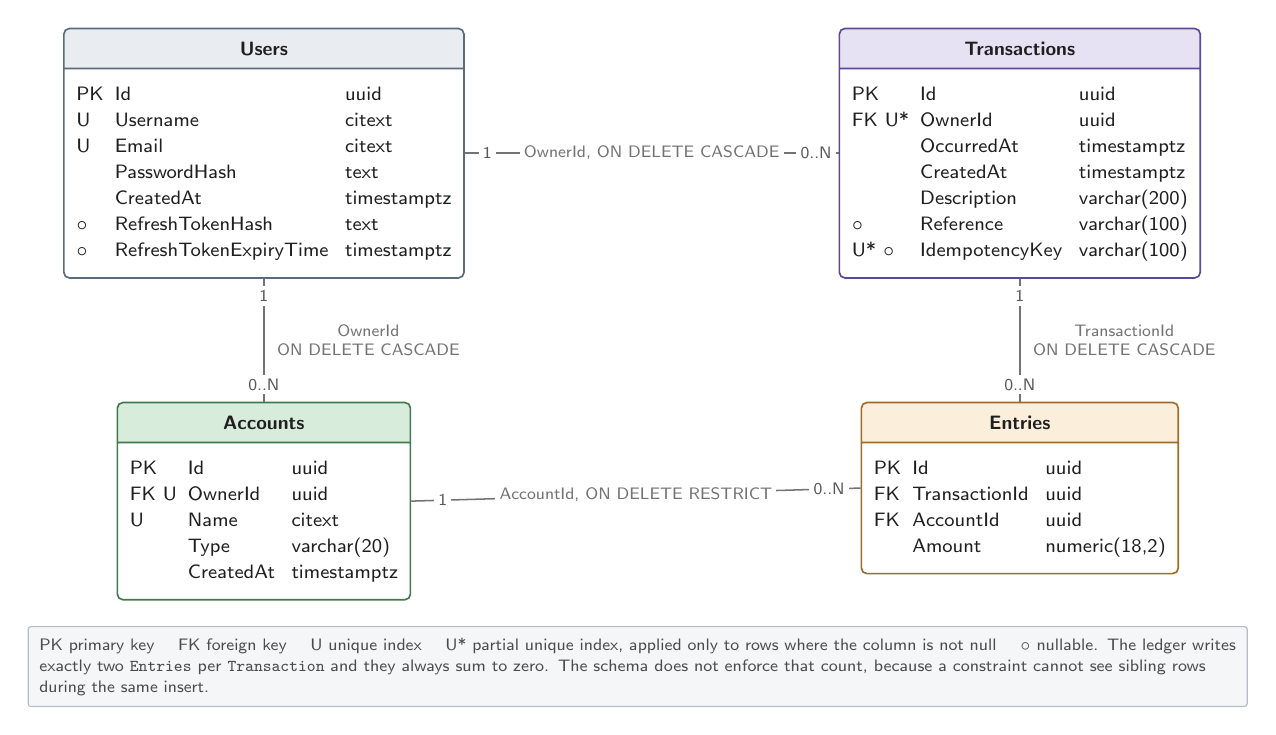
\begin{tikzpicture}[x=1cm,y=1cm,
  ent/.style={rectangle split,rectangle split parts=2,draw,line width=0.6pt,
    rounded corners=2pt,font=\sffamily\fontsize{6.8}{8}\selectfont,
    text=black!88,inner sep=4.5pt,anchor=north},
  rel/.style={line width=0.55pt,draw=black!55},
  card/.style={font=\sffamily\fontsize{6}{7}\selectfont,text=black!65,
    inner sep=1.5pt,fill=white},
  fk/.style={font=\sffamily\fontsize{5.8}{7}\selectfont,text=black!55,
    inner sep=1.5pt,fill=white,align=center}]

  \node[ent,rectangle split part fill={cActorF,white},draw=cActorL] (users) at (3.0,0)
   {\textbf{Users}\nodepart{two}
    \begin{tabular}{@{}l@{\hspace{4pt}}l@{\hspace{6pt}}l@{}}
      PK & Id & uuid\\
      U  & Username & citext\\
      U  & Email & citext\\
         & PasswordHash & text\\
         & CreatedAt & timestamptz\\
      $\circ$ & RefreshTokenHash & text\\
      $\circ$ & RefreshTokenExpiryTime & timestamptz\\
    \end{tabular}};

  \node[ent,rectangle split part fill={cDbF,white},draw=cDbL] (tx) at (12.6,0)
   {\textbf{Transactions}\nodepart{two}
    \begin{tabular}{@{}l@{\hspace{4pt}}l@{\hspace{6pt}}l@{}}
      PK & Id & uuid\\
      FK U* & OwnerId & uuid\\
         & OccurredAt & timestamptz\\
         & CreatedAt & timestamptz\\
         & Description & varchar(200)\\
      $\circ$ & Reference & varchar(100)\\
      U* $\circ$ & IdempotencyKey & varchar(100)\\
    \end{tabular}};

  \node[ent,rectangle split part fill={cApiF,white},draw=cApiL] (acc) at (3.0,-4.75)
   {\textbf{Accounts}\nodepart{two}
    \begin{tabular}{@{}l@{\hspace{4pt}}l@{\hspace{6pt}}l@{}}
      PK & Id & uuid\\
      FK U & OwnerId & uuid\\
      U & Name & citext\\
        & Type & varchar(20)\\
        & CreatedAt & timestamptz\\
    \end{tabular}};

  \node[ent,rectangle split part fill={cCliF,white},draw=cCliL] (ent) at (12.6,-4.75)
   {\textbf{Entries}\nodepart{two}
    \begin{tabular}{@{}l@{\hspace{4pt}}l@{\hspace{6pt}}l@{}}
      PK & Id & uuid\\
      FK & TransactionId & uuid\\
      FK & AccountId & uuid\\
         & Amount & numeric(18,2)\\
    \end{tabular}};

  \draw[rel] (users.south) -- node[card,pos=0.14]{1} node[card,pos=0.86]{0..N}
    node[fk,pos=0.5,anchor=west,xshift=3pt]{OwnerId\\ON DELETE CASCADE} (acc.north);
  \draw[rel] (users.east) -- node[card,pos=0.06]{1} node[card,pos=0.94]{0..N}
    node[fk,pos=0.5]{OwnerId, ON DELETE CASCADE} (tx.west);
  \draw[rel] (acc.east) -- node[card,pos=0.07]{1} node[card,pos=0.93]{0..N}
    node[fk,pos=0.5]{AccountId, ON DELETE RESTRICT} (ent.west);
  \draw[rel] (tx.south) -- node[card,pos=0.14]{1} node[card,pos=0.86]{0..N}
    node[fk,pos=0.5,anchor=west,xshift=3pt]{TransactionId\\ON DELETE CASCADE} (ent.north);

  \node[notebox,text width=15.2cm,anchor=north west] at (0.0,-7.6)
   {PK primary key \quad FK foreign key \quad U unique index \quad
    U* partial unique index, applied only to rows where the column is not null
    \quad $\circ$ nullable.
    The ledger writes exactly two \texttt{Entries} per \texttt{Transaction} and
    they always sum to zero. The schema does not enforce that count, because a
    constraint cannot see sibling rows during the same insert.};
\end{tikzpicture}
\caption{The four tables, their keys and their delete rules. Balances are absent
by design: an account balance is \texttt{SUM(Amount)} over its entries.}
\label{fig:er}
\end{figure}

The two referential actions differ deliberately. Deletion of a transaction
cascades to its entries, because an entry without its header carries no meaning.
Deletion of an account that has been posted to is refused by
\code{ON DELETE RESTRICT}, because such a deletion would destroy history and
unbalance every transaction in which the account appears.

\code{Account.Type} is stored by name rather than by ordinal, through
\code{HasConversion<string>()} in the model and \code{JsonStringEnumConverter}
on the wire. Reordering the \code{AccountType} enumeration would otherwise
reinterpret every stored row and every value already sent to a client.

Three indexes serve a functional purpose rather than a performance one. The
unique index on \code{(OwnerId, Name)} prevents two concurrent requests from
creating the same account twice. The partial unique index on
\code{(OwnerId, IdempotencyKey)} performs the equivalent function for duplicate
postings, and is partial so that the many transactions carrying no key do not
collide with one another. The composite index on
\code{(OwnerId, OccurredAt, CreatedAt)} matches the ordering used by every
listing.

% ================================================================ SECTION 4
\section{Principal code components}

\subsection{Backend}

The backend is organised into four layers, each holding a single
responsibility. A request enters at a controller, which reads the caller's
identity and determines the response shape. Controllers issue no queries. A
service owns the business rules and the queries. \code{AppDbContext} owns the
schema. The data transfer objects own validation. Table~\ref{tab:backend}
lists the files of the backend.

{\setlength{\LTpre}{8pt}\setlength{\LTpost}{8pt}
\begin{longtable}{@{}p{5.0cm}p{10.0cm}@{}}
\caption{Principal files of the backend and their responsibilities.}
\label{tab:backend}\\
\toprule
\textbf{\sffamily\small File} & \textbf{\sffamily\small Responsibility}\\
\midrule
\endfirsthead
\caption[]{Principal files of the backend and their responsibilities. (continued)}\\
\toprule
\textbf{\sffamily\small File} & \textbf{\sffamily\small Responsibility}\\
\midrule
\endhead
\bottomrule
\endlastfoot
\code{Program.cs} &
  Service registration and middleware ordering. Applies pending migrations at
  startup, configures JWT validation with \code{ClockSkew} set to zero, and
  installs the rate limiter and the global exception handler.\\
\code{Controllers/} &
  Six endpoints for accounts, three for transactions and five for
  authentication. Each reads \code{User.GetUserId()} from the validated token
  and delegates to a service.\\
\code{AuthService.cs} &
  Registration, sign in, renewal and sign out. Owns BCrypt hashing, refresh
  token generation and rotation, and access token construction.\\
\code{AccountService.cs} &
  The chart of accounts, per account statements with a running balance, and the
  trial balance. Balances are produced by a correlated subquery in
  \code{WithBalance}.\\
\code{TransactionService.cs} &
  The write path: idempotency resolution, the account ownership check, the
  overdraft check with its row lock, and the single batched save.\\
\code{Data/AppDbContext.cs} &
  The complete schema, comprising indexes, check constraints, referential
  actions and the \code{citext} extension. EF Core derives the migrations from
  it.\\
\code{DTOs/} &
  Request and response shapes. The write objects carry the validation
  attributes and, where a rule spans more than one field, an
  \code{IValidatableObject} method.\\
\code{ValidateModelAttribute.cs} &
  Registered globally, so that no controller repeats the model state check and
  no controller can omit it.\\
\code{Controllers/ApiResponse.cs} &
  The response envelope returned by every endpoint, for success and failure
  alike.\\
\end{longtable}}

Two helpers merit specific mention. \code{ConfigurationExtensions.Require}
raises an exception when a configuration key is absent, so a deployment lacking a
signing key or a connection string terminates at startup and names the missing
value, rather than failing later on its first query or issuing tokens signed with
an empty key. \code{ClaimsPrincipalExtensions.GetUserId} reads the subject claim
from the validated token and is the sole means by which a service learns who is
calling.

\subsection{Frontend}

Table~\ref{tab:frontend} lists the files of the frontend.

{\setlength{\LTpre}{8pt}\setlength{\LTpost}{8pt}
\begin{longtable}{@{}p{5.0cm}p{10.0cm}@{}}
\caption{Principal files of the frontend and their responsibilities.}
\label{tab:frontend}\\
\toprule
\textbf{\sffamily\small File} & \textbf{\sffamily\small Responsibility}\\
\midrule
\endfirsthead
\caption[]{Principal files of the frontend and their responsibilities. (continued)}\\
\toprule
\textbf{\sffamily\small File} & \textbf{\sffamily\small Responsibility}\\
\midrule
\endhead
\bottomrule
\endlastfoot
\code{proxy.ts} &
  Executes before matched requests. Redirects according to session state and
  renews an access token approaching expiry, rewriting the request's own cookie
  header so that the render below it uses the new value.\\
\code{lib/auth.ts} &
  Cookie names and attributes, session read and write, and decoding of the
  access token claims. Marked \code{server-only}.\\
\code{lib/api.ts} &
  The sole location from which an HTTP call to the API is issued.
  \code{apiFetch} does not raise and always returns the envelope.
  \code{apiFetchAuthed} attaches the caller's own token and accepts no user
  identifier parameter.\\
\code{lib/ledger.ts} &
  Typed wrappers for the five read endpoints, together with the TypeScript
  counterparts of the API data transfer objects.\\
\code{app/(auth)/actions.ts} &
  The \code{login}, \code{register} and \code{signOut} Server Actions.\\
\code{app/dashboard/*/actions.ts} &
  \code{createAccount} and \code{postTransaction}. Both invoke
  \code{revalidatePath} on success, so that the pages affected by a write are
  rebuilt.\\
\code{app/dashboard/*/page.tsx} &
  Server Components. Each awaits its data and returns completed markup.\\
\code{lib/use-dialog.ts} &
  Dialog open state that closes only once the server confirms the submission,
  so that a rejected submission retains every value the user entered.\\
\end{longtable}}

The types in \code{lib/ledger.ts} are written by hand rather than generated.
Five small types impose a lower reading cost than a code generation step, and a
divergence from the API surfaces as a type error at the point of use.

% ================================================================ SECTION 5
\section{Internal operation of the API}

\subsection{Request processing pipeline}

Every request traverses the same ordered sequence of middleware before a
controller receives it. The order is declared in \code{Program.cs} and is
significant: each stage may terminate the request, and a stage placed too late
cannot protect the stages above it. Figure~\ref{fig:pipeline} states the
sequence together with the function of each stage.

\begin{figure}[H]
\centering
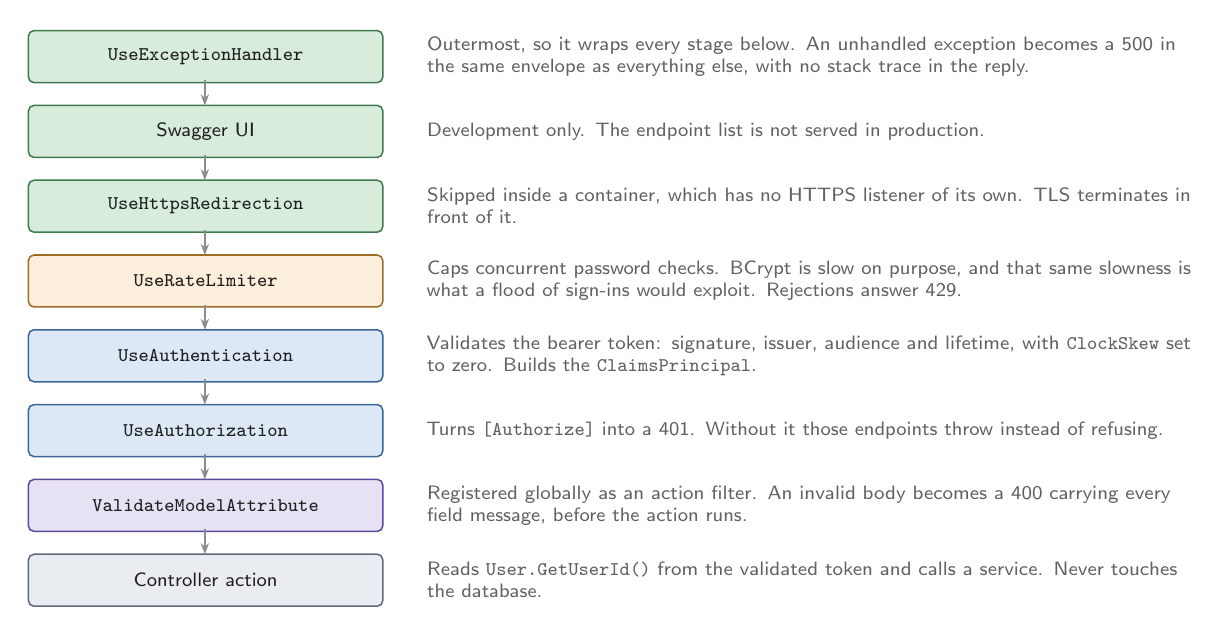
\begin{tikzpicture}[x=1cm,y=1cm,
  st/.style={draw,rounded corners=2pt,line width=0.55pt,minimum width=4.5cm,
    minimum height=0.66cm,font=\sffamily\fontsize{7.2}{8.4}\selectfont,
    text=black!88,inner sep=3pt,anchor=west},
  ann/.style={font=\sffamily\fontsize{6.8}{8}\selectfont,text=black!62,
    anchor=west,align=left,text width=9.7cm}]

  \foreach \y/\f/\d/\t/\a in {
    0/cApiF/cApiL/{\texttt{UseExceptionHandler}}/{Outermost, so it wraps every stage below. An unhandled exception becomes a 500 in the same envelope as everything else, with no stack trace in the reply.},
    -0.95/cApiF/cApiL/{Swagger UI}/{Development only. The endpoint list is not served in production.},
    -1.90/cApiF/cApiL/{\texttt{UseHttpsRedirection}}/{Skipped inside a container, which has no HTTPS listener of its own. TLS terminates in front of it.},
    -2.85/cCliF/cCliL/{\texttt{UseRateLimiter}}/{Caps concurrent password checks. BCrypt is slow on purpose, and that same slowness is what a flood of sign-ins would exploit. Rejections answer 429.},
    -3.80/cBffF/cBffL/{\texttt{UseAuthentication}}/{Validates the bearer token: signature, issuer, audience and lifetime, with \texttt{ClockSkew} set to zero. Builds the \texttt{ClaimsPrincipal}.},
    -4.75/cBffF/cBffL/{\texttt{UseAuthorization}}/{Turns \texttt{[Authorize]} into a 401. Without it those endpoints throw instead of refusing.},
    -5.70/cDbF/cDbL/{\texttt{ValidateModelAttribute}}/{Registered globally as an action filter. An invalid body becomes a 400 carrying every field message, before the action runs.},
    -6.65/cActorF/cActorL/{Controller action}/{Reads \texttt{User.GetUserId()} from the validated token and calls a service. Never touches the database.}}
    {\node[st,fill=\f,draw=\d] at (0,\y) {\t};
     \node[ann] at (4.95,\y) {\a};}

  \foreach \y in {-0.3,-1.25,-2.2,-3.15,-4.1,-5.05,-6.0}
    {\draw[-{Stealth[length=4pt]},line width=0.5pt,draw=black!45] (2.25,\y) -- (2.25,\y-0.32);}
\end{tikzpicture}
\caption{The middleware order in \texttt{Program.cs}. A request enters at the
top; anything that fails is answered from the stage that caught it.}
\label{fig:pipeline}
\end{figure}

\subsection{Uniform response envelope}

Every endpoint returns \code{ApiResponse<T>} for both success and failure. The
envelope carries \code{success}, \code{message}, \code{data}, \code{errors},
\code{statusCode} and \code{timeStamp}. Validation failures use it, the rate
limiter uses it, and the global exception handler uses it.

The consequence on the frontend is substantial. \code{apiFetch} in
\code{lib/api.ts} does not raise. An unreachable API is caught and converted
into the same envelope with status 503, and a response body that is not an
envelope is converted likewise. Every caller therefore requires exactly one
branch:

\begin{lstlisting}
const result = await apiFetchAuthed<Transaction>("/api/transactions", { ... });
if (!result.success || !result.data) { return { message: result.message, ... }; }
\end{lstlisting}

No second error path and no \code{try}/\code{catch} block is required at any
call site. The framework's automatic 400 response is disabled in
\code{Program.cs} for the same reason, since it returns a \code{ProblemDetails}
document that does not conform to this shape.

\subsection{Request validation}

Validation is declared on the data transfer objects and nowhere else. Rules
governing a single field are expressed as attributes. Rules that read more than
one field are expressed in an \code{IValidatableObject} method, because no
single attribute can span two properties. \code{TransactionWriteDto} declares
two such rules: the debit and credit accounts must differ, and the date may not
exceed the current time by more than one day.

The frontend does not restate these rules. The forms carry
\code{noValidate} and the actions transmit the values as entered. The messages
produced by the API are presented to the user unaltered. Two copies of a
validation rule diverge over time, at which point the copy the user sees is no
longer the copy that governs the outcome.

One field is deliberately exempt from normalisation. \code{Username},
\code{Email}, \code{Description} and \code{Reference} are trimmed in their
property setters. \code{Password} is not. It is supplied to
\code{BCrypt.HashPassword} and \code{BCrypt.Verify} exactly as the user entered
it, including any leading or trailing whitespace, because trimming would
produce a stored credential that the user cannot reproduce.

Dates are normalised in the service rather than in the data transfer object.
\code{AsUtc} converts a local value and labels an unspecified one as UTC rather
than converting it, because the form submits midnight UTC for a calendar day and
a conversion would move the posting to the adjacent day.

\subsection{Authentication and session management}

Sign in returns two tokens with distinct functions. The access token is a JSON
Web Token signed with HMAC SHA512, valid for 15 minutes, carrying the user
identifier, the username and a unique token identifier. The API stores no
record of it. Its signature constitutes the proof of issuance, and validating
that signature is a local computation requiring no database access.

The refresh token consists of 32 bytes drawn from the cryptographic random
number generator. It carries no information, and only a SHA256 digest of it is
stored on the user row alongside an expiry seven days forward. It is rotated on
every use.

The two are hashed by different algorithms for a specific reason. A password is
hashed with BCrypt, which is deliberately slow, because a human selected
password is drawn from a small set of probable values and the cost of each
attempt is what renders exhaustive search impractical. A refresh token consists
of 256 random bits with no probable values, so a deliberately slow hash would
provide no additional resistance while imposing a cost on every renewal. SHA256
is therefore the appropriate choice.

Sign out clears the stored refresh token digest on the server and subsequently
deletes the cookies. Clearing the digest is the decisive step, because renewal compares an incoming token against that stored
value. Once it is null, every copy of that refresh token is invalid, not only
the copy held by the browser that issued the request.

The stored digest is compared using \code{CryptographicOperations.FixedTimeEquals}
rather than an ordinary string comparison. An ordinary comparison returns at the
first differing byte, and that timing difference would allow the correct value to
be recovered one byte at a time.

Figure~\ref{fig:signin} traces the sign in sequence from the form submission to
the rendered dashboard.

\begin{figure}[H]
\centering
\def\sqbot{-12.75}
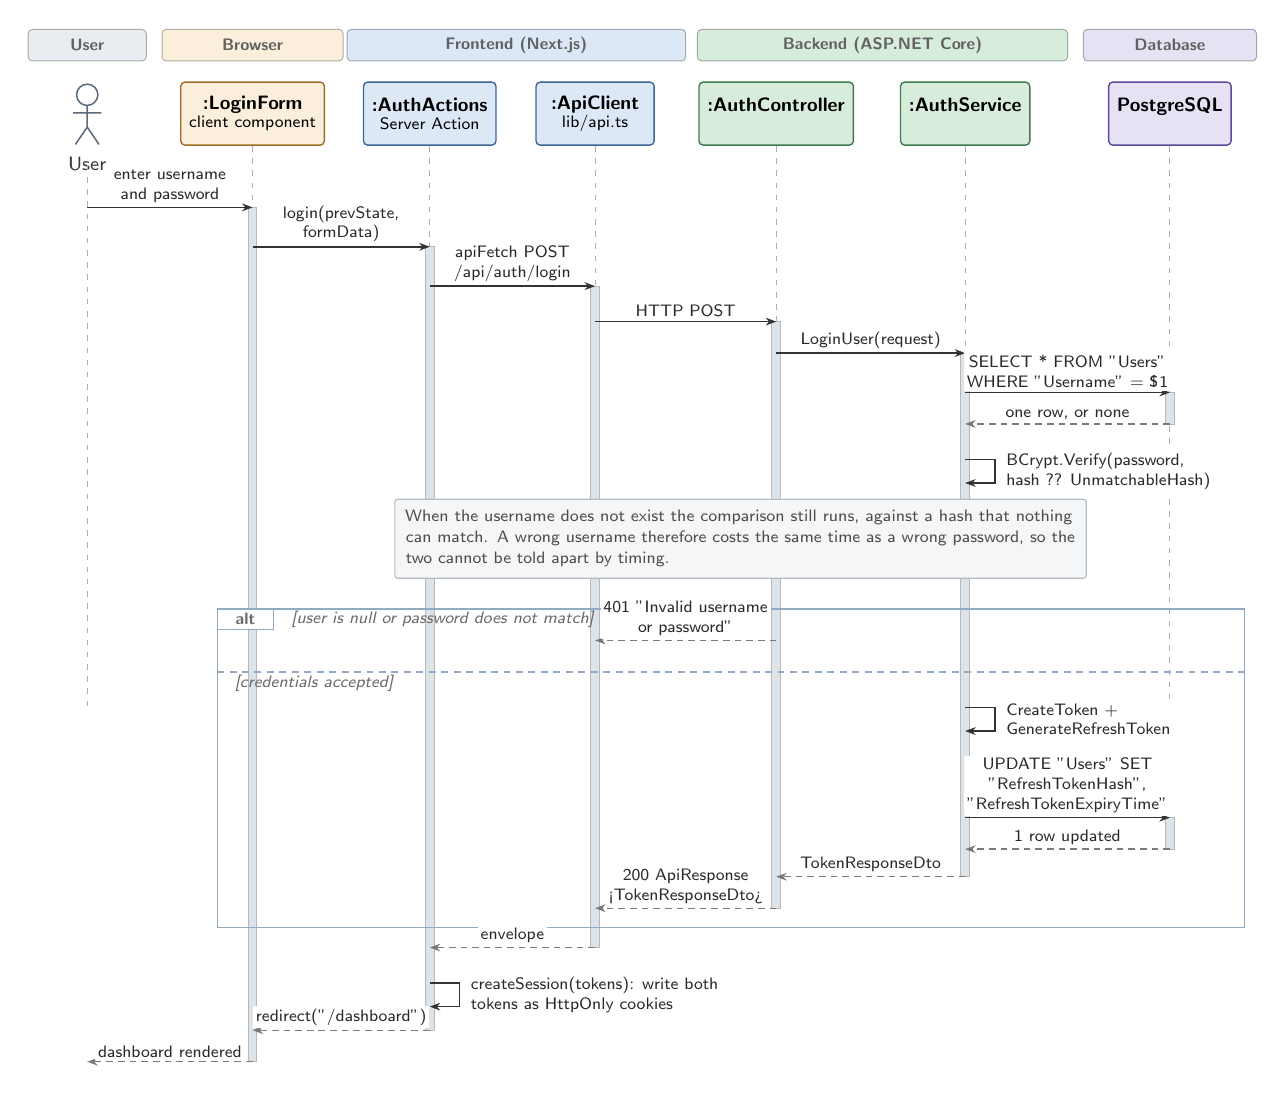
\begin{tikzpicture}[x=1cm,y=1cm]
  \band{-0.10}{1.40}{cActorF}{User}
  \band{1.60}{3.90}{cCliF}{Browser}
  \band{3.95}{8.25}{cBffF}{Frontend (Next.js)}
  \band{8.40}{13.10}{cApiF}{Backend (ASP.NET Core)}
  \band{13.30}{15.50}{cDbF}{Database}

  \actorfig{0.65}{User}
  \lifeline{2.75}{lf}{sqclient}{:LoginForm}{client component}
  \lifeline{5.00}{aa}{sqbff}{:AuthActions}{Server Action}
  \lifeline{7.10}{ac}{sqbff}{:ApiClient}{lib/api.ts}
  \lifeline{9.40}{ct}{sqapi}{:AuthController}{}
  \lifeline{11.80}{sv}{sqapi}{:AuthService}{}
  \lifeline{14.40}{db}{sqdb}{PostgreSQL}{}

  \act{2.75}{-1.60}{-12.45}\act{5.00}{-2.10}{-12.05}\act{7.10}{-2.60}{-11.00}
  \act{9.40}{-3.05}{-10.50}\act{11.80}{-3.45}{-10.10}
  \act{14.40}{-3.95}{-4.35}\act{14.40}{-9.35}{-9.75}

  \msg{0.65}{2.75}{-1.60}{enter username\\and password}
  \msg{2.75}{5.00}{-2.10}{login(prevState,\\formData)}
  \msg{5.00}{7.10}{-2.60}{apiFetch POST\\/api/auth/login}
  \msg{7.10}{9.40}{-3.05}{HTTP POST}
  \msg{9.40}{11.80}{-3.45}{LoginUser(request)}
  \msg{11.80}{14.40}{-3.95}{SELECT * FROM "Users"\\WHERE "Username" = \$1}
  \ret{14.40}{11.80}{-4.35}{one row, or none}
  \selfmsg{11.80}{-4.80}{BCrypt.Verify(password,\\hash ?? UnmatchableHash)}
  \sqnote{4.55}{-5.30}{8.5cm}{When the username does not exist the comparison still
    runs, against a hash that nothing can match. A wrong username therefore costs
    the same time as a wrong password, so the two cannot be told apart by timing.}

  \frag{2.30}{-6.70}{15.35}{-10.75}{alt}{[user is null or password does not match]}
  \ret{9.40}{7.10}{-7.10}{401 "Invalid username\\or password"}
  \draw[sqfrag,dash pattern=on 2.5pt off 2pt] (2.30,-7.50) -- (15.35,-7.50);
  \node[font=\sffamily\fontsize{6}{6.8}\selectfont\itshape,text=black!58,anchor=west]
    at (2.40,-7.64) {[credentials accepted]};

  \selfmsg{11.80}{-7.95}{CreateToken +\\GenerateRefreshToken}
  \msg{11.80}{14.40}{-9.35}{UPDATE "Users" SET\\"RefreshTokenHash",\\"RefreshTokenExpiryTime"}
  \ret{14.40}{11.80}{-9.75}{1 row updated}
  \ret{11.80}{9.40}{-10.10}{TokenResponseDto}
  \ret{9.40}{7.10}{-10.50}{200 ApiResponse\\<TokenResponseDto>}
  \ret{7.10}{5.00}{-11.00}{envelope}
  \selfmsg{5.00}{-11.45}{createSession(tokens): write both\\tokens as HttpOnly cookies}
  \ret{5.00}{2.75}{-12.05}{redirect("/dashboard")}
  \ret{2.75}{0.65}{-12.45}{dashboard rendered}
\end{tikzpicture}
\caption{Signing in. Both tokens stop at the Next.js server and become HttpOnly
cookies. The browser receives a rendered dashboard and never holds a credential.}
\label{fig:signin}
\end{figure}

\subsection{Authorization and query scoping}\label{sec:authz}

Authentication establishes who is calling. Authorization restricts what that
caller can reach, and in this system it is enforced by the way queries are
constructed rather than by a check applied to their results. Both services
declare a single scoping method and every read begins from it:

\begin{lstlisting}
private IQueryable<Transaction> OwnedBy(Guid ownerId) =>
    _appDbContext.Transactions.Where(transaction => transaction.OwnerId == ownerId);
\end{lstlisting}

The owner identifier is supplied by \code{User.GetUserId()}, which reads the
subject claim of the validated token. No endpoint accepts a user identifier as
a parameter, so no caller can express a request on another user's behalf. The
consequence is that a query returning another user's rows cannot be written
without first removing the scoping method, rather than merely forgetting a
check. Writes are scoped by the same value, which the service stamps on the row
instead of accepting it from the request body.

A resource belonging to another user is reported as absent rather than
forbidden. \code{GetAccount} returns null for both conditions and the
controller answers 404 in either case, so the response cannot be used to
determine which identifiers exist.

\subsection{Recording a transaction}

This write path is the only one whose correctness depends on the order in which
its operations are performed.
The \code{CreateTransaction} method of \code{TransactionService} performs five
operations in a fixed sequence, which Figure~\ref{fig:post} sets out in full.

\begin{figure}[H]
\centering
\def\sqbot{-13.20}
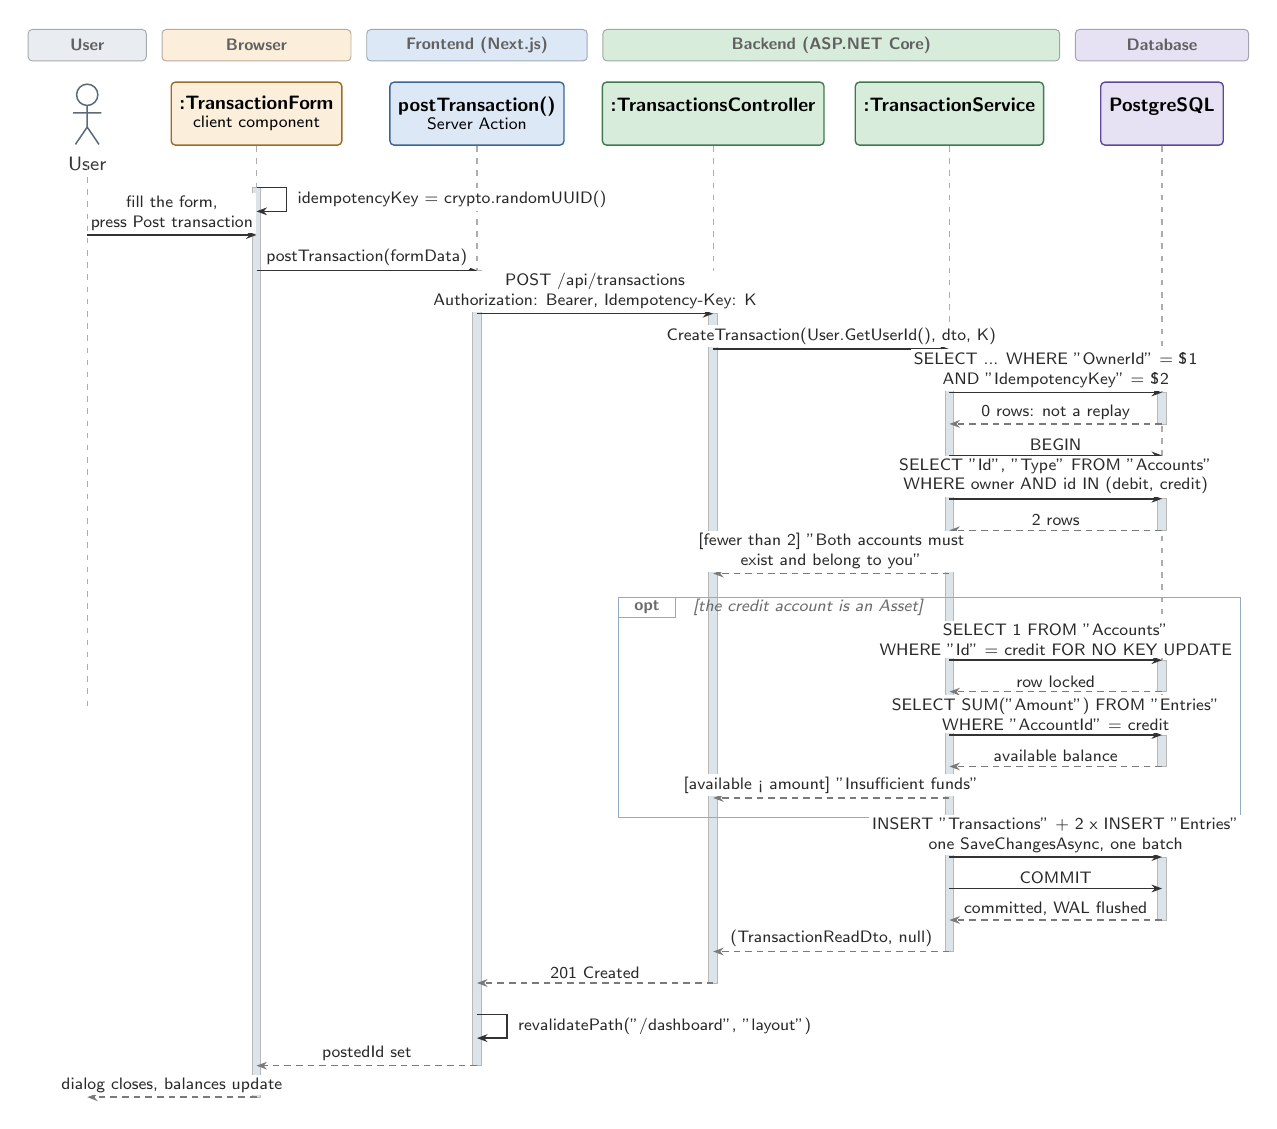
\begin{tikzpicture}[x=1cm,y=1cm]
  \band{-0.10}{1.40}{cActorF}{User}
  \band{1.60}{4.00}{cCliF}{Browser}
  \band{4.20}{7.00}{cBffF}{Frontend (Next.js)}
  \band{7.20}{13.00}{cApiF}{Backend (ASP.NET Core)}
  \band{13.20}{15.40}{cDbF}{Database}

  \actorfig{0.65}{User}
  \lifeline{2.80}{tf}{sqclient}{:TransactionForm}{client component}
  \lifeline{5.60}{pa}{sqbff}{postTransaction()}{Server Action}
  \lifeline{8.60}{ct}{sqapi}{:TransactionsController}{}
  \lifeline{11.60}{sv}{sqapi}{:TransactionService}{}
  \lifeline{14.30}{db}{sqdb}{PostgreSQL}{}

  \act{2.80}{-1.35}{-12.90}\act{5.60}{-2.40}{-12.50}
  \act{8.60}{-2.95}{-11.45}\act{11.60}{-3.40}{-11.05}
  \act{14.30}{-3.95}{-4.35}\act{14.30}{-5.30}{-5.70}
  \act{14.30}{-7.35}{-7.75}\act{14.30}{-8.30}{-8.70}
  \act{14.30}{-9.85}{-10.65}

  \selfmsg{2.80}{-1.35}{idempotencyKey = crypto.randomUUID()}
  \msg{0.65}{2.80}{-1.95}{fill the form,\\press Post transaction}
  \msg{2.80}{5.60}{-2.40}{postTransaction(formData)}
  \msg{5.60}{8.60}{-2.95}{POST /api/transactions\\Authorization: Bearer, Idempotency-Key: K}
  \msg{8.60}{11.60}{-3.40}{CreateTransaction(User.GetUserId(), dto, K)}
  \msg{11.60}{14.30}{-3.95}{SELECT ... WHERE "OwnerId" = \$1\\AND "IdempotencyKey" = \$2}
  \ret{14.30}{11.60}{-4.35}{0 rows: not a replay}
  \msg{11.60}{14.30}{-4.75}{BEGIN}
  \msg{11.60}{14.30}{-5.30}{SELECT "Id", "Type" FROM "Accounts"\\WHERE owner AND id IN (debit, credit)}
  \ret{14.30}{11.60}{-5.70}{2 rows}
  \ret{11.60}{8.60}{-6.25}{[fewer than 2] "Both accounts must\\exist and belong to you"}

  \frag{7.40}{-6.55}{15.30}{-9.35}{opt}{[the credit account is an Asset]}
  \msg{11.60}{14.30}{-7.35}{SELECT 1 FROM "Accounts"\\WHERE "Id" = credit FOR NO KEY UPDATE}
  \ret{14.30}{11.60}{-7.75}{row locked}
  \msg{11.60}{14.30}{-8.30}{SELECT SUM("Amount") FROM "Entries"\\WHERE "AccountId" = credit}
  \ret{14.30}{11.60}{-8.70}{available balance}
  \ret{11.60}{8.60}{-9.10}{[available < amount] "Insufficient funds"}

  \msg{11.60}{14.30}{-9.85}{INSERT "Transactions" + 2 x INSERT "Entries"\\one SaveChangesAsync, one batch}
  \msg{11.60}{14.30}{-10.25}{COMMIT}
  \ret{14.30}{11.60}{-10.65}{committed, WAL flushed}
  \ret{11.60}{8.60}{-11.05}{(TransactionReadDto, null)}
  \ret{8.60}{5.60}{-11.45}{201 Created}
  \selfmsg{5.60}{-11.85}{revalidatePath("/dashboard", "layout")}
  \ret{5.60}{2.80}{-12.50}{postedId set}
  \ret{2.80}{0.65}{-12.90}{dialog closes, balances update}
\end{tikzpicture}
\caption{Posting a transaction. The idempotency key is settled before any lock
is taken, and the header and both entries are written by a single
\texttt{SaveChangesAsync} inside one database transaction.}
\label{fig:post}
\end{figure}

The idempotency key is resolved first, before the database transaction is
opened. A replayed request should incur no cost and must not queue behind an
active posting against the same account.

The account lookup serves two purposes in a single query. It confirms that
both accounts exist, and because the query filters on \code{OwnerId} it
confirms that both belong to the caller. A result of fewer than two rows
indicates that at least one account is absent or owned by another user. Both
conditions produce an identical message, so the response cannot be used to
determine which account identifiers exist.

The overdraft check executes only when the credit account is of type Asset.
That restriction is deliberate. An Asset is the only account type for which a
negative balance indicates an error. Liability, Income and Equity accounts are
credit normal and hold negative balances in the ordinary course, so a floor
applied to them would reject correct bookkeeping.

The header and both entries are written by one \code{SaveChangesAsync} call
inside one database transaction. Section~\ref{sec:acid} sets out the atomicity
that this provides.

\subsection{Reading the ledger}

Reads are projected rather than materialised. Each query ends in
\code{ProjectTo}, which compiles the AutoMapper configuration into the SQL
select list, so only the columns the data transfer object declares are
retrieved and no entity is tracked by the change tracker. Balances are produced
by the correlated subquery in \code{WithBalance}, which keeps a listing of any
length to one statement rather than one statement per account.

Transaction history is paged by the API rather than by the client. The page
number and size are bounded by \code{Range} attributes, the size to 100, and the
count is taken before the slice so that the total describes the whole result
rather than the page returned. \code{TotalPages} is derived from the count and
the size rather than stored, so the two cannot disagree. The offset is computed
as a 64 bit value:

\begin{lstlisting}
var skip = (long)(page - 1) * pageSize;
if (skip >= totalCount) { return new PaginatedResult<TransactionReadDto> { ... }; }
\end{lstlisting}


The running balance on an account statement is accumulated in application code
over the ordered projection rather than computed by a window function. The
order is fixed by \code{OccurredAt} and then \code{CreatedAt}, the same order
the composite index provides, so the accumulation follows the sequence the rows
are already returned in.

\subsection{Idempotent submission}\label{sec:idem}

An HTTP client that receives no response cannot determine what occurred. The
request may have been lost in transit, or the response may have been lost after
the transaction was committed. Retransmission is the only available remedy, and
in the absence of protection a retransmission records the posting a second
time.

The browser generates a UUID when the form mounts and transmits it in the
\code{Idempotency-Key} header. The key is replaced only after a confirmed
success, which constitutes the entire mechanism:

\begin{lstlisting}
useEffect(() => { setIdempotencyKey(crypto.randomUUID()); }, [state.postedId]);
\end{lstlisting}

\code{state.postedId} changes only when the API confirms a posting. A failed
attempt leaves it unchanged, the effect does not re-execute, and the
retransmission carries the same key. Generating a new key on failure would
convert every retransmission into a second genuine transaction.

The API examines the key before writing. That examination does not itself
constitute the guarantee. Two requests carrying the same key may both complete
the examination before either has committed, and both will find no existing
row.

The losing request rolls back before reading. This ordering is required: after
a failed statement PostgreSQL marks the transaction as aborted and rejects any
subsequent query on it until the rollback is issued. The sequence is therefore
rollback, re-read, and return the row written by the winner. Both callers
receive the same transaction and exactly one row exists.

Figure~\ref{fig:idem} sets out the resulting interleaving.

\begin{figure}[!htbp]
\centering
\def\sqbot{-8.70}
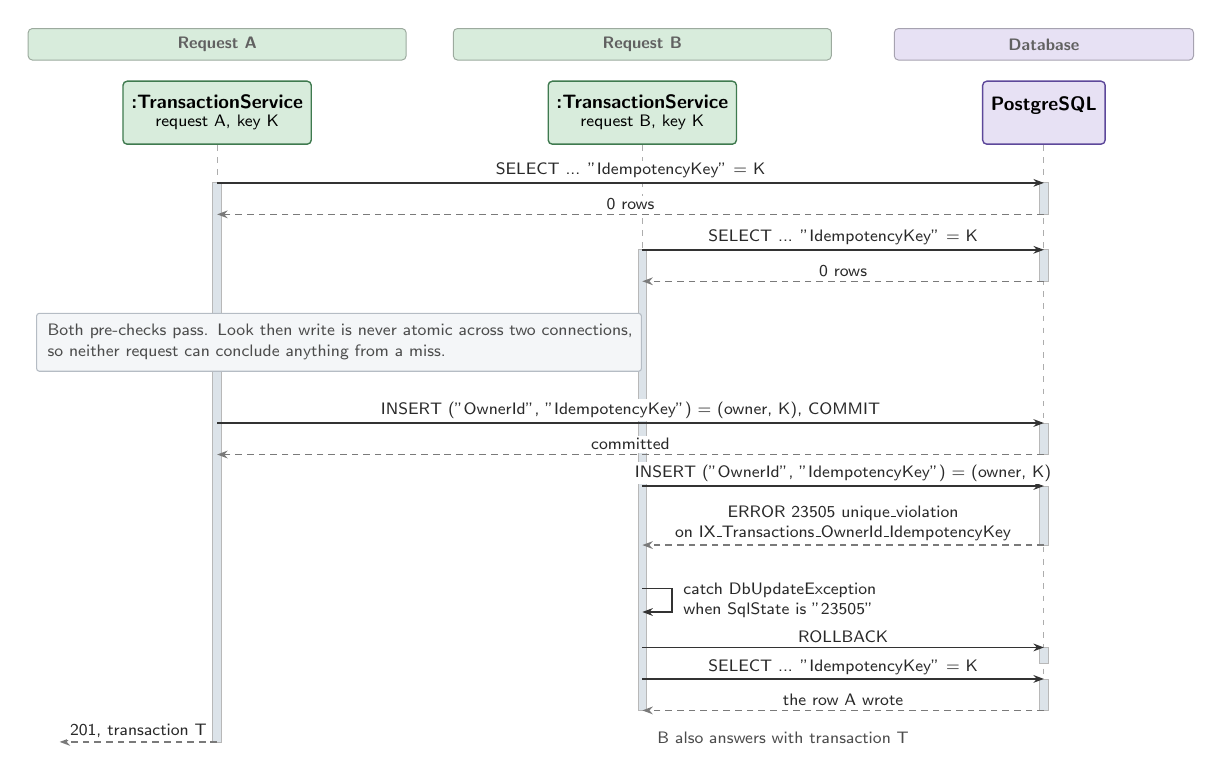
\begin{tikzpicture}[x=1cm,y=1cm]
  \band{0.60}{5.40}{cApiF}{Request A}
  \band{6.00}{10.80}{cApiF}{Request B}
  \band{11.60}{15.40}{cDbF}{Database}

  \lifeline{3.00}{a}{sqapi}{:TransactionService}{request A, key K}
  \lifeline{8.40}{b}{sqapi}{:TransactionService}{request B, key K}
  \lifeline{13.50}{db}{sqdb}{PostgreSQL}{}

  \act{3.00}{-1.30}{-8.40}\act{8.40}{-2.15}{-8.00}
  \act{13.50}{-1.30}{-1.70}\act{13.50}{-2.15}{-2.55}
  \act{13.50}{-4.35}{-4.75}\act{13.50}{-5.15}{-5.90}
  \act{13.50}{-7.20}{-7.40}\act{13.50}{-7.60}{-8.00}

  \msg{3.00}{13.50}{-1.30}{SELECT ... "IdempotencyKey" = K}
  \ret{13.50}{3.00}{-1.70}{0 rows}
  \msg{8.40}{13.50}{-2.15}{SELECT ... "IdempotencyKey" = K}
  \ret{13.50}{8.40}{-2.55}{0 rows}

  \sqnote{0.70}{-2.95}{7.4cm}{Both pre-checks pass. Look then write is never
    atomic across two connections, so neither request can conclude anything from
    a miss.}

  \msg{3.00}{13.50}{-4.35}{INSERT ("OwnerId", "IdempotencyKey") = (owner, K), COMMIT}
  \ret{13.50}{3.00}{-4.75}{committed}
  \msg{8.40}{13.50}{-5.15}{INSERT ("OwnerId", "IdempotencyKey") = (owner, K)}
  \ret{13.50}{8.40}{-5.90}{ERROR 23505 unique\_violation\\on IX\_Transactions\_OwnerId\_IdempotencyKey}
  \selfmsg{8.40}{-6.45}{catch DbUpdateException\\when SqlState is "23505"}
  \msg{8.40}{13.50}{-7.20}{ROLLBACK}
  \msg{8.40}{13.50}{-7.60}{SELECT ... "IdempotencyKey" = K}
  \ret{13.50}{8.40}{-8.00}{the row A wrote}
  \ret{3.00}{1.00}{-8.40}{201, transaction T}
  \node[sqfree,anchor=west,text=black!70] at (8.55,-8.35)
    {B also answers with transaction T};
\end{tikzpicture}
\caption{Two requests carrying one idempotency key. The partial unique index is
the guarantee; PostgreSQL evaluates it inside the commit, where nothing can slip
between the look and the write.}
\label{fig:idem}
\end{figure}

\subsection{Row level locking}\label{sec:lock}

Derived balances remove most contention from the system. A posting does not need to read the current balance before deciding what to write. Therefore, concurrent postings can simply append their entries, and the final balance remains correct regardless of which transaction is considered first.

The overdraft rule is different. It must first read the balance, check whether the withdrawal is allowed, and then write the new entries. Between these steps, another transaction may change the balance. For example, if an account has 100 and two concurrent withdrawals of 60 both read the balance as 100, both may pass the overdraft check and commit. The final balance then becomes $-20$. This is a form of write skew that can occur under Read Committed isolation.

To prevent this, the credit account row is locked before checking its balance. The second transaction must wait until the first transaction finishes. Once it obtains the lock, it reads the updated balance of 40 instead of 100 and therefore rejects the second withdrawal. The lock is acquired inside the same database transaction as the entry insertion, so it remains held until the transaction commits.

The lock mode used is \code{FOR NO KEY UPDATE} instead of \code{FOR UPDATE}. This is important because inserting an \code{Entry} also causes PostgreSQL to acquire an implicit \code{FOR KEY SHARE} lock on the referenced \code{Accounts} row. This lock ensures that the referenced account cannot be deleted or have its key changed while the entry is being inserted. As a result, every posting involves both account rows: one through the explicit lock and the other through the foreign key.

The choice of lock mode also matters for transfers in opposite directions. Suppose one transaction transfers money from A to B while another transfers money from B to A. With \code{FOR UPDATE}, each transaction explicitly locks one account and then requires a \code{FOR KEY SHARE} lock on the other account through the foreign key. These locks can conflict with the lock already held by the other transaction, causing both transactions to wait for each other.

With \code{FOR NO KEY UPDATE}, the situation is different. The implicit \code{FOR KEY SHARE} lock is compatible with the explicit lock, so the foreign key check does not create this conflict. At the same time, two transactions trying to acquire \code{FOR NO KEY UPDATE} on the same account still conflict with each other and therefore wait in sequence. This provides the required serialization for concurrent withdrawals without introducing the unnecessary conflict between transfers in opposite directions.



\subsection{Transactional guarantees and concurrency control}\label{sec:acid}

The ledger depends on the four transactional properties commonly abbreviated
ACID. This section states how each is obtained and which component is
responsible for it.

\subsubsection*{Atomicity}

A posting consists of three rows: one \code{Transactions} row and two
\code{Entries} rows. \code{CreateTransaction} opens an explicit database
transaction with \code{BeginTransactionAsync} before any of them is constructed,
EF Core emits all three inserts from one \code{SaveChangesAsync} call as a
single batch within that transaction, and \code{CommitAsync} makes them visible
together. No concurrent reader can observe a debit without its credit, because
no such state is ever committed.

Every exit path discards the work. The transaction is declared with
\code{await using}, so disposal occurs on every return, and disposing an
uncommitted transaction rolls it back. The ownership failure and the
insufficient funds refusal both return early and are covered by this. The
duplicate key case is handled explicitly, because the subsequent read must
occur on a usable connection:

\begin{lstlisting}
await using var dbTransaction = await _appDbContext.Database.BeginTransactionAsync();
...
try { await _appDbContext.SaveChangesAsync(); await dbTransaction.CommitAsync(); }
catch (DbUpdateException ex) when (key != null
       && ex.InnerException is PostgresException { SqlState: "23505" })
{
    await dbTransaction.RollbackAsync();
    return (await FindByIdempotencyKey(ownerId, key), null);
}
\end{lstlisting}

\subsubsection*{Consistency}

Consistency requires that a committed transaction leave the database satisfying
every declared invariant. The invariants are declared in \code{AppDbContext}
and enforced by PostgreSQL, so they hold irrespective of the code path that
reaches the table. They are the check constraints, unique indexes and
referential actions set out in Section~\ref{sec:schema}.

One invariant is established by construction rather than by the schema. The two
entries of a posting are created as \code{+amount} and \code{-amount} within one
object graph, so their sum is necessarily zero. No check constraint can express
this, because a constraint is evaluated against a single row while the invariant
spans two rows written in the same batch. The trial balance aggregates the same
quantity across every account, so the equality of its totals verifies the
invariant continuously rather than by a separate calculation.

The overdraft rule is an application level invariant rather than a schema level
one, for the same reason: it constrains an aggregate over many rows, which no
row constraint can evaluate.

\subsubsection*{Isolation}

The database operates at PostgreSQL's default isolation level, Read Committed.
Each statement observes a snapshot taken when that statement began, so no
statement reads uncommitted data and readers are never blocked by writers.

The choice has a direct consequence for reporting. \code{GetTrialBalance}
delegates to \code{GetAccounts}, which projects every balance as a correlated
subquery within one \code{SELECT}. The whole trial balance is therefore computed
from a single statement and a single snapshot, and cannot observe a posting in a
partially applied state, even though the isolation level would permit two
separate statements to disagree.

Read Committed permits non-repeatable reads, phantom rows and write skew.
Of these, only write skew affects correctness here, and it arises on exactly one
code path, which the row lock of Section~5.7 covers. The stronger levels were
considered and rejected on the following grounds.

Serializable would remove the write skew without an explicit lock, but it
detects conflicts rather than preventing them: it aborts one transaction with
SQLSTATE \code{40001} at commit time, after the work has been performed, which
obliges every caller to implement retry logic. Repeatable Read imposes the same
requirement and does not prevent write skew in any case, and optimistic
concurrency using a version column likewise discovers the conflict only after
the work is complete. Read Committed with one row lock on the single path that
reads before it writes is the narrower arrangement.

\subsubsection*{Durability}

\code{COMMIT} returns only after the corresponding write ahead log record has
been flushed to durable storage. PostgreSQL enables \code{synchronous\_commit}
by default, so a transaction reported as committed survives an immediate loss of
power to the database process.

Container durability is provided by the named volume \code{pgdata}, which holds
the data directory outside the container filesystem. The database container may
be replaced or rebuilt without loss, and only \code{docker compose down -v}
removes the volume.

\subsubsection*{Concurrency control}

Two situations require explicit control: a decision taken on a value that
another transaction may change before the write lands, and two requests
competing to create the same uniquely identified row. Table~\ref{tab:conc}
enumerates every instance of both in the system.

\begin{table}[!htbp]
\caption{Concurrent conflicts arising in the system and the mechanism that
resolves each.}
\label{tab:conc}
\centering
\begin{tabular}{@{}R{3.3cm}R{4.4cm}p{6.8cm}@{}}
\toprule
\textbf{\sffamily\small Conflict} & \textbf{\sffamily\small Origin} &
\textbf{\sffamily\small Resolving mechanism}\\
\midrule
Duplicate posting &
  Retransmission after a lost response, or two browser tabs &
  Partial unique index on \code{(OwnerId, IdempotencyKey)}. The violation is
  caught as SQLSTATE \code{23505}, the transaction is rolled back, and the
  committed row is returned.\\
Duplicate account name &
  Two concurrent create requests from one owner &
  Unique index on \code{(OwnerId, Name)}, reported to the caller as 409.\\
Duplicate registration &
  Two concurrent sign ups &
  Unique indexes on \code{Username} and \code{Email}, reported as 409.\\
Overdraft through write skew &
  Two withdrawals from one Asset account &
  \code{FOR NO KEY UPDATE} on the credit row, held until commit. The second
  request waits and then reads the updated balance.\\
Lock cycle &
  Two transfers posted in opposite directions &
  The explicit mode is chosen so that the implicit foreign key lock does not
  conflict with it, so no wait-for cycle can form.\\
Exhaustion by password hashing &
  A burst of sign in or registration requests &
  Concurrency limiter on the bcrypt policy, which bounds simultaneous
  verifications and answers 429 beyond the queue limit.\\
\bottomrule
\end{tabular}
\end{table}

The first three cases share one structure: the application checks before
writing, but the index is what decides. The check only improves the error
message, for the reason given in Section~\ref{sec:idem}.

% ================================================================ SECTION 6
\section{Containerization}

\code{docker compose up --build} starts three containers. The database becomes
available first, the API waits until the database is accepting connections, and
the Next.js server waits until the API is serving requests.
Figure~\ref{fig:docker} states the topology and the startup dependencies.

\begin{figure}[H]
\centering
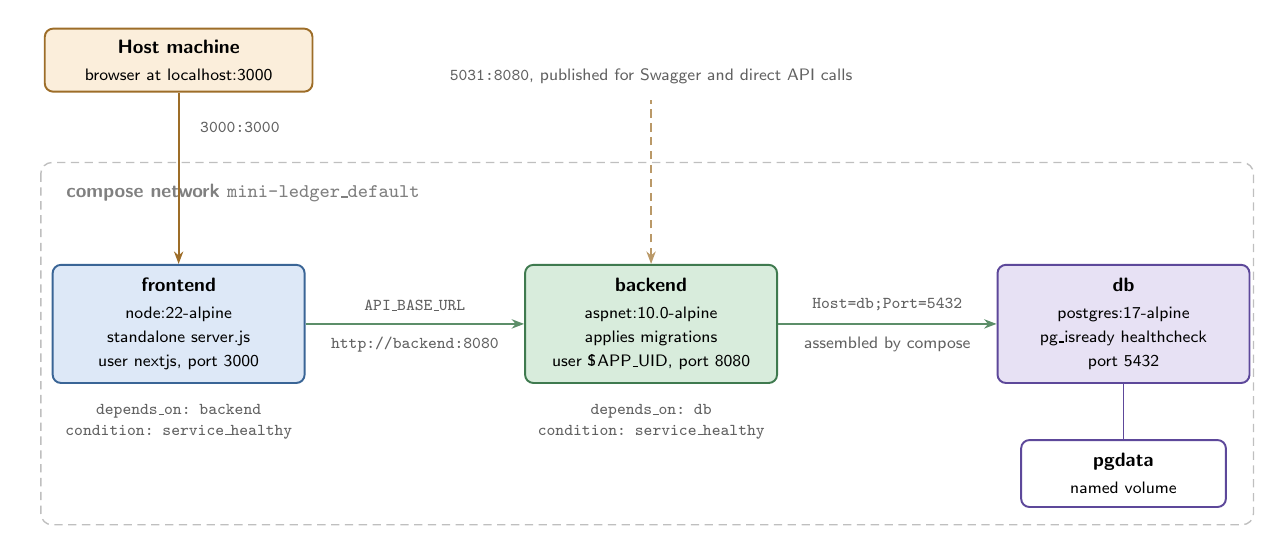
\begin{tikzpicture}[x=1cm,y=1cm,
  ct/.style={draw,rounded corners=3pt,line width=0.7pt,align=center,
    font=\sffamily\fontsize{7.4}{8.8}\selectfont,minimum width=3.2cm,
    minimum height=1.5cm,inner sep=4pt},
  lbl/.style={font=\sffamily\fontsize{6.4}{7.4}\selectfont,text=black!62,align=center},
  dep/.style={-{Stealth[length=4.5pt]},line width=0.7pt,draw=cApiL!85}]

  \draw[draw=black!25,line width=0.5pt,rounded corners=4pt,dash pattern=on 3pt off 2pt]
    (0.15,-0.55) rectangle (15.55,-5.15);
  \node[font=\sffamily\fontsize{6.6}{7.6}\selectfont\bfseries,text=black!50,anchor=north west]
    at (0.35,-0.70) {compose network \texttt{mini-ledger\_default}};

  \node[ct,fill=cBffF,draw=cBffL] (fe) at (1.90,-2.60)
    {\textbf{frontend}\\[1pt]\sub{node:22-alpine}\\\sub{standalone server.js}\\\sub{user nextjs, port 3000}};
  \node[ct,fill=cApiF,draw=cApiL] (be) at (7.90,-2.60)
    {\textbf{backend}\\[1pt]\sub{aspnet:10.0-alpine}\\\sub{applies migrations}\\\sub{user \$APP\_UID, port 8080}};
  \node[ct,fill=cDbF,draw=cDbL] (dbc) at (13.90,-2.60)
    {\textbf{db}\\[1pt]\sub{postgres:17-alpine}\\\sub{pg\_isready healthcheck}\\\sub{port 5432}};

  \draw[dep] (fe.east) -- node[lbl,above=1pt,midway]{\texttt{API\_BASE\_URL}}
    node[lbl,below=1pt,midway]{\texttt{http://backend:8080}} (be.west);
  \draw[dep] (be.east) -- node[lbl,above=1pt,midway]{\texttt{Host=db;Port=5432}}
    node[lbl,below=1pt,midway]{assembled by compose} (dbc.west);

  \node[lbl,anchor=north,text width=3.6cm] at (1.90,-3.50)
    {\texttt{depends\_on: backend}\\\texttt{condition: service\_healthy}};
  \node[lbl,anchor=north,text width=3.6cm] at (7.90,-3.50)
    {\texttt{depends\_on: db}\\\texttt{condition: service\_healthy}};

  \node[ct,fill=white,draw=cDbL,minimum width=2.6cm,minimum height=0.85cm]
    (vol) at (13.90,-4.50) {\textbf{pgdata}\\[1pt]\sub{named volume}};
  \draw[line width=0.6pt,draw=cDbL] (dbc.south) -- (vol.north);

  \node[ct,fill=cCliF,draw=cCliL,minimum width=3.4cm,minimum height=0.8cm]
    (host) at (1.90,0.75) {\textbf{Host machine}\\[1pt]\sub{browser at localhost:3000}};
  \draw[{Stealth[length=4.5pt]}-,line width=0.7pt,draw=cCliL] (fe.north) -- (host.south);
  \node[lbl,anchor=west] at (2.05,-0.10) {\texttt{3000:3000}};

  \draw[{Stealth[length=4.5pt]}-,line width=0.6pt,draw=cCliL!70,dash pattern=on 3pt off 2pt]
    (be.north) -- (7.90,0.25);
  \node[lbl,anchor=south] at (7.90,0.32)
    {\texttt{5031:8080}, published for Swagger and direct API calls};
\end{tikzpicture}
\caption{The three containers. Only the frontend needs to be reachable from the
host; the backend port is published for convenience, not because the browser
uses it.}
\label{fig:docker}
\end{figure}

\subsection{Image construction}

Both images are built in multiple stages. The API is compiled with
\code{mcr.microsoft.com\brk/dotnet\brk/sdk:10.0-alpine} and shipped on
\code{mcr.microsoft.com\brk/dotnet\brk/aspnet:10.0-alpine}. The runtime image carries
the .NET runtime without a compiler, so neither source code nor build tooling
is present in the published image.

The restore step is separated from the source copy so that the layer cache
remains effective:

\begin{lstlisting}
COPY backend.csproj .
RUN dotnet restore
COPY . .
RUN dotnet publish -c Release -o /app --no-restore
\end{lstlisting}

Modifying a \code{.cs} file invalidates only the final two instructions. The
package download is reused until \code{backend.csproj} itself changes.

The Next.js image is built in three stages. \code{deps} executes \code{npm ci},
which installs precisely the lockfile and fails if the lockfile and the manifest
disagree; \code{builder} executes \code{next build}; \code{runner} copies
\code{.next/standalone} and \code{.next/static} only. The standalone output
traces the files the server reaches at runtime and emits a minimal
\code{node\_modules}, so \code{typescript}, \code{tailwindcss}, \code{postcss}
and \code{shadcn} are present at build time and absent at runtime.

Both runtime images execute as a non root user. The API uses the
\code{\$APP\_UID} account defined by its base image, and the Next.js image
creates \code{nextjs} with uid 1001. Neither process writes to the container
filesystem, so neither is granted the ability to do so. This also determines the
listening port: the API listens on 8080 rather than 80, because binding a port
below 1024 requires a privilege that the non root account does not hold.

One instruction in the API image addresses a specific defect:

\begin{lstlisting}
RUN apk add --no-cache krb5-libs
\end{lstlisting}

Npgsql probes for Kerberos authentication support when opening a connection.
Alpine does not ship that library, so in its absence every startup emits a
failure to load \code{libgssapi\_krb5.so.2}. The connection succeeds
regardless, but a spurious error line in the startup log is a worse outcome
than the two megabytes the package occupies.

\subsection{Service startup ordering}

\code{depends\_on} combined with \code{condition: service\_healthy} performs a
functional role rather than a decorative one. PostgreSQL starts, executes its
initialisation scripts, and then restarts before it is genuinely ready. Waiting
for the port alone would allow the API to connect during that interval and
fail. \code{pg\_isready} reports actual readiness.

The API declares its own healthcheck against \code{/health}, an anonymous
endpoint that deliberately performs no database access. It answers a single
question: whether this process is serving requests.
\code{docker compose up -d} returns as soon as a container starts, which
precedes Kestrel binding its port, so in the absence of this check the Next.js
server could start against an API that is not yet accepting connections.

The API applies pending migrations at startup:

\begin{lstlisting}
await using (var scope = app.Services.CreateAsyncScope())
{
    await scope.ServiceProvider.GetRequiredService<AppDbContext>().Database.MigrateAsync();
}
\end{lstlisting}

A container starts against an empty database, so the schema must be created
before the first request arrives. The call is idempotent: against a database
already at the latest migration it performs no work, which is what makes
restarting safe.

\subsection{Configuration and secrets}

Secrets are supplied through a \code{.env} file excluded from version control.
\code{.env.example} is the committed template and contains no real values.
Compose performs the substitution and assembles the API connection string from
the same variables used to create the database container, so the two cannot
diverge:

\begin{lstlisting}
ConnectionStrings__DefaultConnection:
    "Host=db;Port=5432;Database=${POSTGRES_DB};Username=${POSTGRES_USER};Password=${POSTGRES_PASSWORD}"
AppSettings__Token: ${JWT_SIGNING_KEY}
\end{lstlisting}

The double underscore is the .NET convention for mapping an environment
variable onto a nested configuration key. \code{API\_BASE\_URL} is set to
\code{http://backend:8080}, using the service name rather than localhost,
because each container holds its own loopback address within the network. The
value is read per request on the server, so one Next.js image runs unchanged in
any environment.
\end{document}
